\documentclass{article}
\usepackage[margin=1in]{geometry}
\usepackage{booktabs}
\usepackage{graphicx}
\title{Reporte de carga MQTT}
\author{Autogenerado por mqtt\_stress\_async.py}
\date{}
\begin{document}
\maketitle
\section*{Resumen de la corrida}
\begin{tabular}{ll}\topruleSesión & 20251204-014425-s00000-n00050 \ CSV & ..\textbackslash\{\}20251204-014425-s00000-n00050-metrics.csv \ Dispositivos & 50.000 \ Publicaciones OK & 1.8e+03 \ Publicaciones fallidas & 0.000 \ Latencia promedio (ms) & 4.916 \ Latencia P95 (ms) & 10.427 \ Mensajes por segundo & 8.630 \ Ancho de banda (Mbps) & 0.011 \ Volumen de datos (MB) & 0.270 \ Duración (s) & 208.580 \ \bottomrule\end{tabular}
\subsection*{Gráficos}
\begin{figure}[h]
\centering
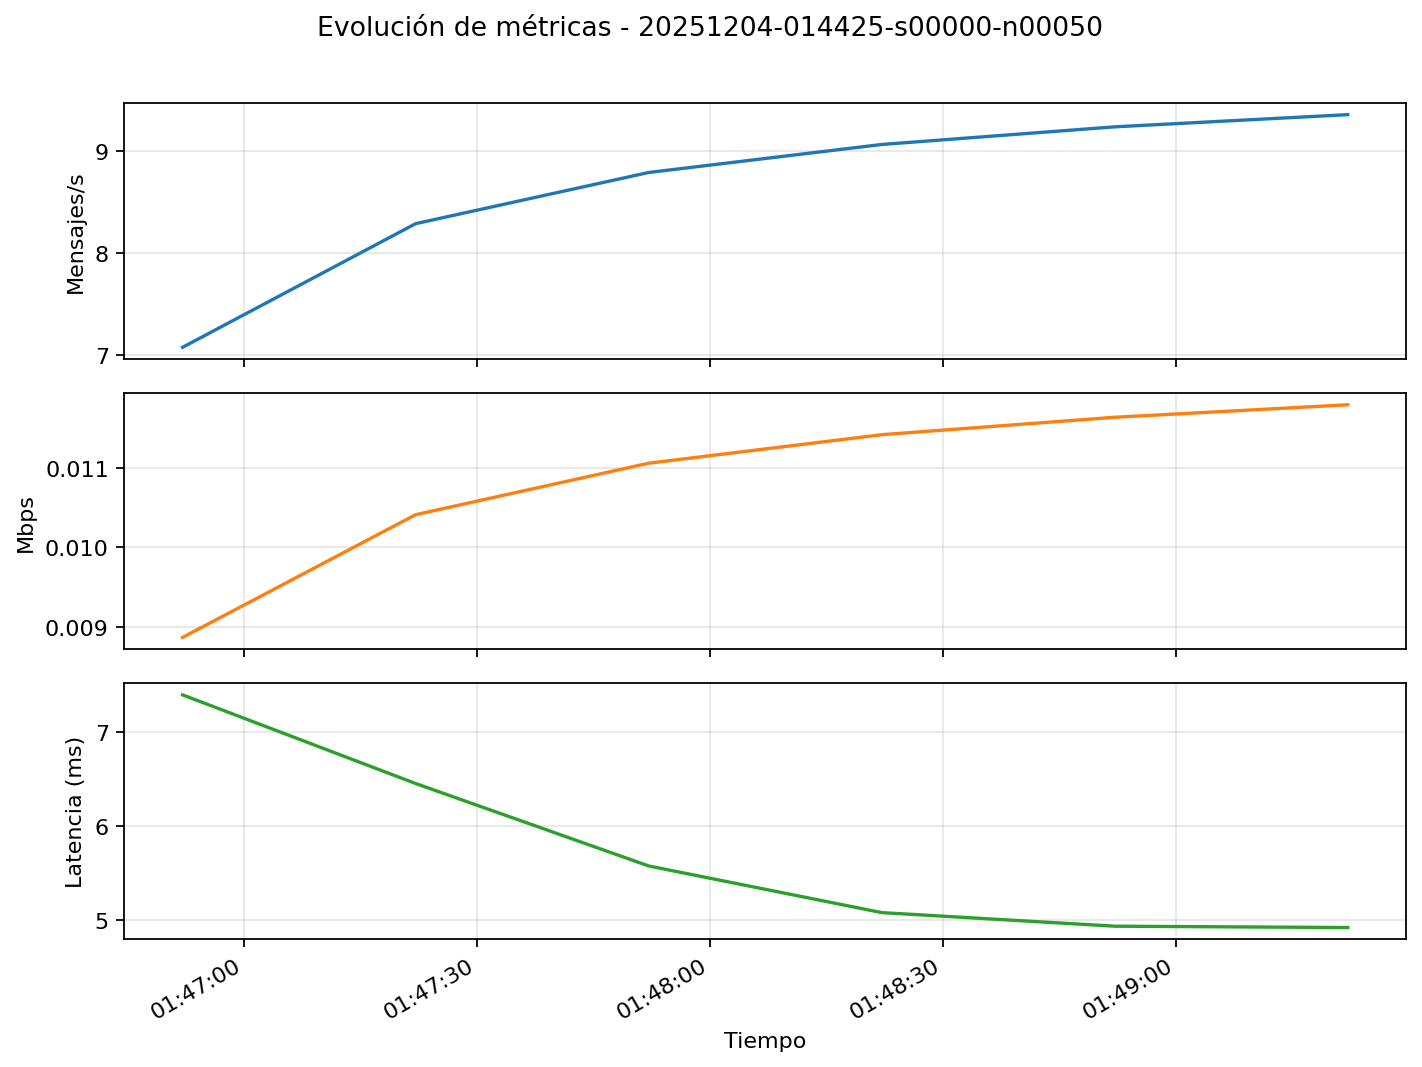
\includegraphics[width=0.9\linewidth]{20251204-014425-s00000-n00050-overview.png}
\caption{Mensajes/s, ancho de banda y latencia promedio.}
\end{figure}

\subsection*{Fuente de datos}
El CSV original se encuentra en \texttt{..\textbackslash\{\}20251204-014425-s00000-n00050-metrics.csv}.\\
Este documento se genera automáticamente tras cada corrida.\
\end{document}
